\section{Aufbau und Durchführung}

\subsection{Aufbau}
\label{sec:Aufbau}

\begin{figure}
    \begin{minipage}[b]{.4\linewidth} % [b] => Ausrichtung an \caption
       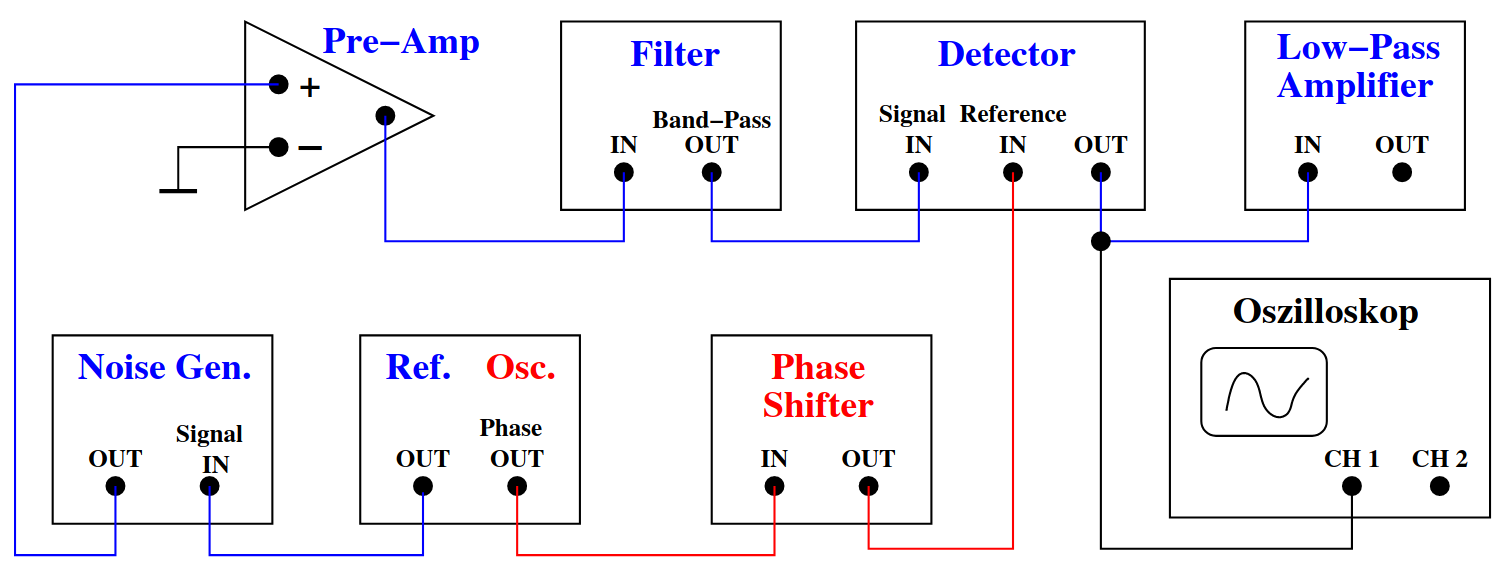
\includegraphics[width=\linewidth]{img/Schema.png}
       \caption{Schematische Darstellung\\ des Lock-In-Verstärkers.\cite{V303}}
       \label{fig:SchematischeDarstellungLockIn}
    \end{minipage}
    \hspace{.1\linewidth}% Abstand zwischen Bilder
    \begin{minipage}[b]{.4\linewidth} % [b] => Ausrichtung an \caption
       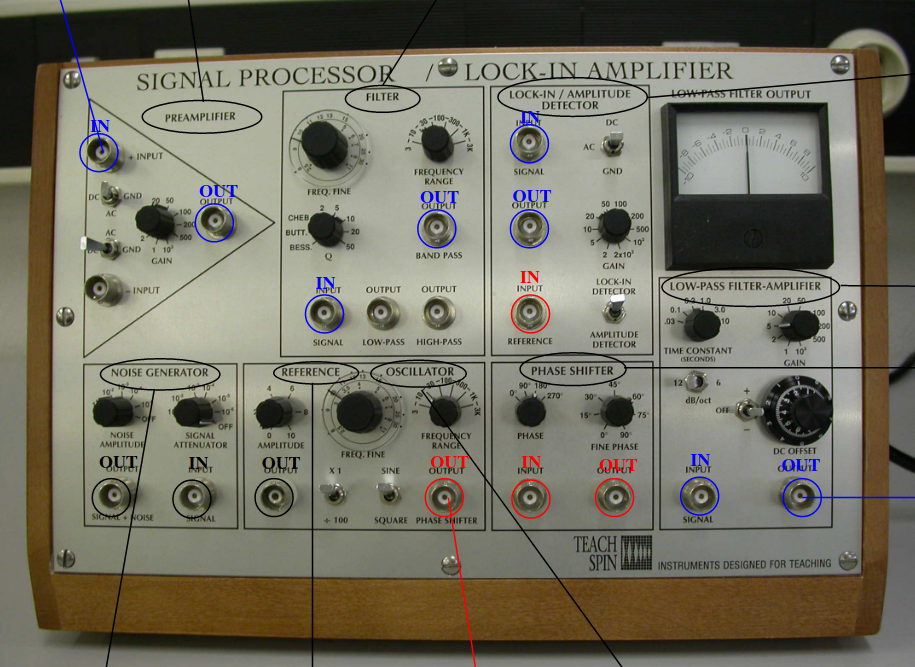
\includegraphics[width=\linewidth]{img/BildLockIn.png}
       \caption{Bild des Lock-In-Verstärkers.\cite{V303}}
       \label{fig:BildLockIn}
    \end{minipage}
 \end{figure}

Für die Versuchsdurchführung wird ein modularer Lock-In-Verstärker und ein Speicher-Oszilloskop verwendet.
Der modulare Verstärker ist in der Abbildung \ref{fig:BildLockIn} zu sehen. Es sind ein Vorverstärker, Hoch-
, Tief- und Bandpassfilter, ein Phasenschieber, ein Funktionsgenerator, ein Rauschgenerator, ein Tiefpass-Verstärker
und ein Amplituden-/ Lock-In-Detektor vorhanden. Die einzelnen Module werden per Kabel miteinander verbunden.

\subsection{Durchführung}
\label{sec:Durchführung}

Für den ersten Teil der Auswertung wird erst der Oscillator- und der Referenceoutput per Kabel an das Oszilloskop angeschlossen. 
Die relevanten Werte werden auf dem Oszillator abgelesen.\\
Für den zweiten Teil der Auswertung werden die Module wie in Abbildung \ref{fig:SchematischeDarstellungLockIn} angeschlossen.
Mit dem Oscillator-Modul wird ein sinusförmiges Signal $U_{sig}$ mit einer Amplitude von etwa 10 mV und einer Frequenz von 1 kHz erzeugt
und an den Verstärker weitergegeben. Der Verstärkerausgang wird mit sinus Referenzsignal $U_{ref}$ mit gleicher Frequenz gemischt.
Um die integrierte Ausgangsspannung zu messen wird der Ausgang des Low-Pass-Verstärkers an den zweiten Kanal des Oszilloskops angeschlossen.\
Die Ausgangssignalskizzen werden per Bildschirmaufnahme angefertigt.\\
Für den dritten Teil der Auswertung wird der Rauschgenerator in der gleichen Größenordnung der Signalspannung $U_{sig}$ angeschlossen.\\
\begin{figure}
    \centering
    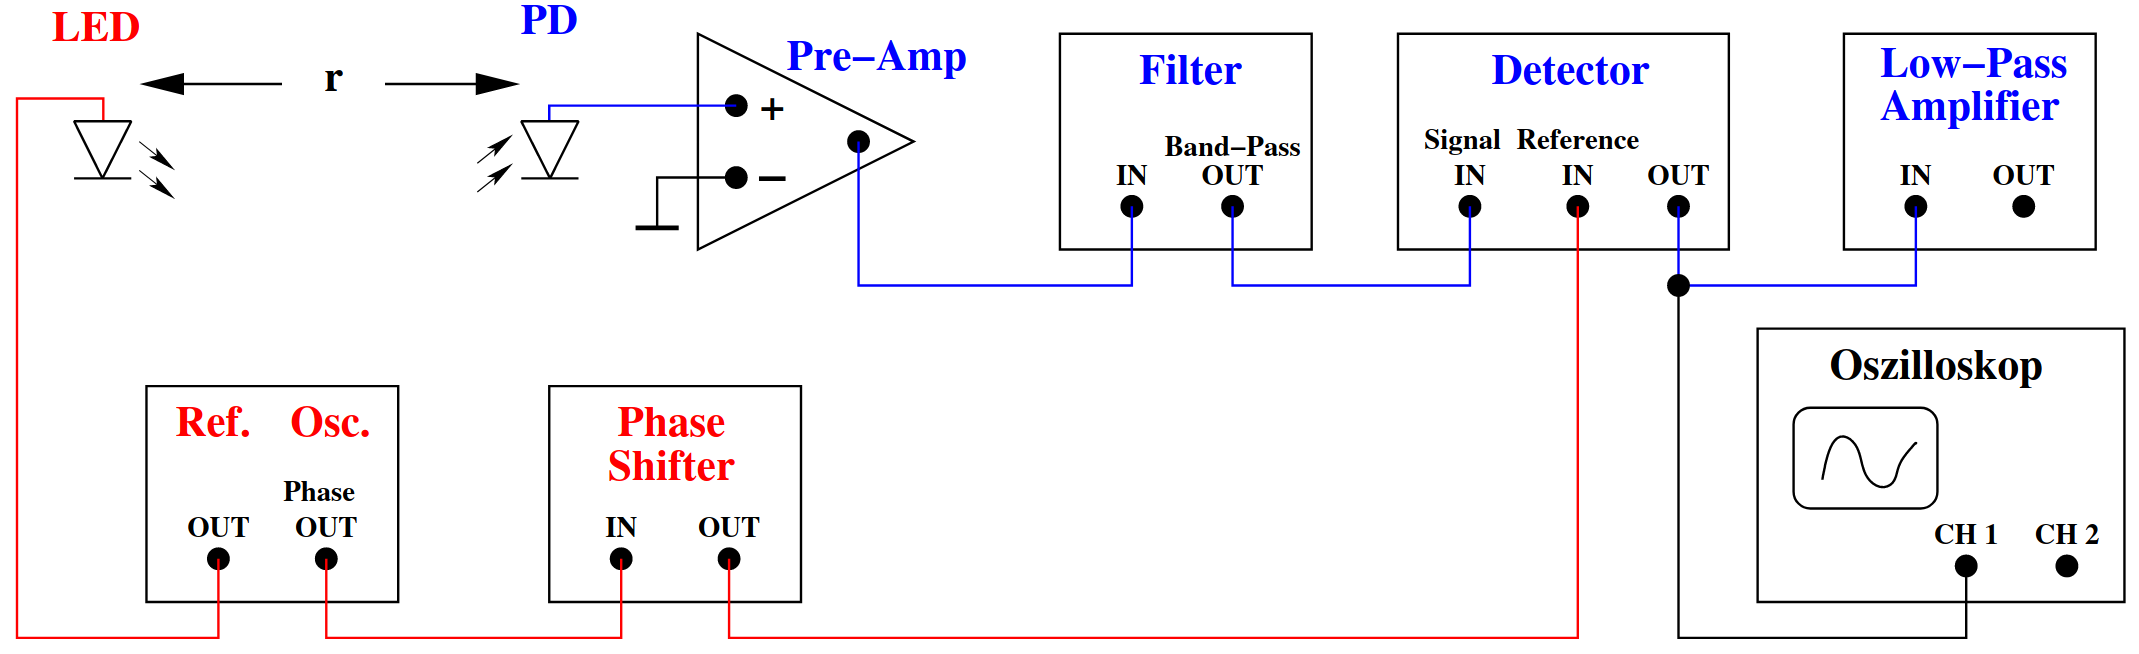
\includegraphics[width=0.7\textwidth]{img/LED.png}
    \caption{Aufbau des Lock-In-Verstärkers mit LED als Rauschgenerator.\cite{V303}}
    \label{fig:LED}
\end{figure}
\\
Für den vierten Teil der Auswertung wird der Rauschgenerator durch eine LED ersetzt. 
Die LED, sowie ein Lichtsensor werden auf einer Schiene befestigt. Während des Versuchs wird die LED immer weiter vom 
Lichtsensor entfernt.
Die Schaltung wird wie in Abbildung \ref{fig:LED} zu sehen aufgebaut.
Die LED wird mithilfe des Reference-Modul mit einer Frequenz von ca 214 Hz angesteuert.
Die Lichtintensität wird wie bei den vorherigen Aufgaben mit dem Tiefpass integriert und auf dem Oszilloskop abgelesen.
Es wird in regelmäßigen Abständen die Spannung gemessen.\\